\documentclass[12pt,letterpaper,noanswers]{exam}
\usepackage[usenames,dvipsnames,svgnames,table]{xcolor}
\usepackage[margin=0.9in]{geometry}
\renewcommand{\familydefault}{\sfdefault}
\usepackage{multicol}
\pagestyle{head}
\header{AM 111 Class 17}{}{Approximating integrals, p.\thepage}
\runningheadrule
\headrule
\usepackage{siunitx}
\usepackage{graphicx} % more modern
\usepackage{amsmath} 
\usepackage{amssymb} 
\usepackage{hyperref}
\usepackage{tcolorbox}
\usepackage{enumitem}
\def\mbf{\mathbf}
\newcommand{\vc}[1]{\boldsymbol{#1}}
\def\dsst{\displaystyle}
\DeclareMathOperator*{\argmin}{arg\,min} % thin space, limits underneath in displays
\usepackage[numbered,autolinebreaks,useliterate]{mcode}

\begin{document}
 \pdfpageheight 11in 
  \pdfpagewidth 8.5in

\noindent 

\section*{Preliminaries}

\begin{itemize}
\itemsep0pt
\item Problem set 07 is due by Friday at 5pm.  Submit extension requests in advance of that time.
\item Your short project proposal is due \textbf{today at 8pm}.
\item There is a skill check in the next class.
\item Regular OH in Pierce G11: today 2-3pm.  OH on Zoom: 3-5pm today.
\end{itemize}


\noindent\textbf{Big picture}

Today: Approximating $\int_{a}^{b}f(x)dx$.

\vspace{0.2cm}
\hrule
\vspace{0.2cm}

\noindent \textbf{Skill check practice}
\begin{questions}
\item %In the figure, the integral $\displaystyle I_{\text{exact}} = \int_0^2 f(x) dx$.  The value of the integral is estimated ($I_\text{estimate}$) via a quadrature rule.  $\displaystyle I_\text{estimate} = \int_0^2 p(x)dx$ for some function $p(x)$.  The function $p(x)$ is shown in black. 

%Answer the following questions about the quadrature rule:

A particular quadrature rule for $\displaystyle\int_0^4f(x)dx$ is given by fitting a parabola to $(0,f(0)), (1,f(1)), (2,f(2))$, fitting a second parabola to $(2,f(2)), (3,f(3)), (4,f(4))$, and integrating the fitted curves.

This is a composite (or adaptive) method:
\begin{oneparchoices}
\choice yes \choice no
\end{oneparchoices}

This is a Newton-Cotes method:
\begin{oneparchoices}
\choice yes \choice no
\end{oneparchoices}

How do you know?

\item The skill from the Class 14 handout (Skill Check C15).
\end{questions}


\vspace{0.2cm}
\hrule
\vspace{0.2cm}

\noindent \textbf{Skill check solution}
\begin{questions}

\item For a composite or adaptive method we would see multiple panels.  A parabola is being fit separately to two sub-regions, so this is a composite method.  

For a Newton-Cotes method, the quadrature points are evenly spaced on the interval, as they are here.

Yes and yes.

\item See the past handout.
\end{questions}
\vspace{0.2cm}
\hrule
\vspace{0.2cm}

\noindent \textbf{Teams}
\begin{multicols}{3}
1. Mina, Basil, Johan

2. Nini, Brian, Eli

3. Nicolas, Aidan, Julia K

4. Mack, Benjamin, Robert

5. Alex, RJ, Jessica

6. Caitlin, Nina, Daniyal

7. Cameron, Dani, Emma

8. Eletria, Julia M, Tom

9. Ray, Ivonne, Shang

10.  Sophie, Eric, Alex

11. Jack, Esmé, Zachary

12. Kevin, Kevin, Marissa

\end{multicols}


%\section*{Numerical Integration}
%\subsection*{Quadrature}
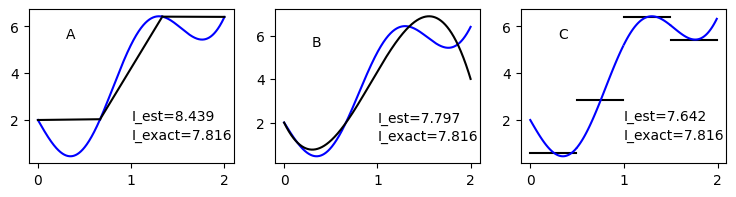
\includegraphics[width=\linewidth]{img/C17estimates.png}
\begin{enumerate}[resume=classQ]
\item In the figure above, the integral $\displaystyle I_{\text{exact}} = \int_0^2 \left(e^x - 2\cos(4x) + 1\right) dx\approx 7.816$.  The value of the integral is estimated via different quadrature rules.  Each estimate is using exactly four function evaluations.
\begin{parts}
\item For each method, $\displaystyle I_\text{estimate} = \int_0^2 p(x)dx$ for some function $p(x)$.  The function $p(x)$ is shown in black for each method.  How many panels appear to be used for each estimate?

\begin{tabular}{c | p{1.5cm} p{1.5cm} p{1.5cm}}
figure &A &B&C \\
\hline
& & & \\
\# panels &\\
&\\
\end{tabular}
\item Assuming there are $k$ function evaluations associated with each panel (some of these function evaluations may be used in multiple panels), identify $k$. 

\begin{tabular}{c | p{1.5cm} p{1.5cm} p{1.5cm}}
figure &A &B&C \\
\hline
& & & \\
$k$ &\\
&\\
\end{tabular}
\item The three quadrature methods used are: composite midpoint, composite trapezoid, Gaussian quadrature on $4$ points.  Match the method to the plot.
\vspace{1in}
\item Which method is most accurate?
\vspace{1cm}
\end{parts}
\end{enumerate}


\subsection*{Monte Carlo integration (see Greenbaum and Chartier \S 3.3)}
\begin{tcolorbox}
\begin{itemize}
\itemsep0em
%\item For many functions, an integral cannot be computed analytically: numerical approximation is the main option in that case.
    \item \textbf{Monte Carlo integration} is an even weight quadrature where the set of nodes is chosen randomly (usually using a uniform distribution over a unit interval or box).
    \item In 1D: $\displaystyle\int_a^b f(x) dx \approx (b-a)\frac{1}{N}\sum\limits_{k=1}^Nf(x_k)$ where $x_k$ is chosen uniformly at random from the interval $[a,b]$
     \item In integrals over 1D or 2D domains, Monte Carlo integration is less efficient than the other quadrature methods we have studied.
      \item The error in the approximation decreases at the rate $1/\sqrt{N}$ where $N$ is the number of points sampled, regardless of dimension, so this technique is very useful for higher dimensional problems.
      \item The \textbf{unit box} in $\mathbb{R}^n$ is $[0,1]\times [0,1] ...\times [0,1] = [0,1]^n$.  In $\mathbb{R}$ this is the unit interval while in $\mathbb{R}^2$ this is the unit square.
    \end{itemize}
    \end{tcolorbox}


\noindent\textbf{Monte Carlo quadrature points for a double integral}

%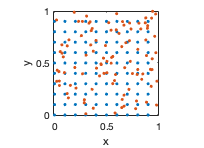
\includegraphics{img/C15domain.png}

\begin{multicols}{2}
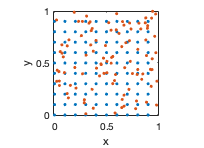
\includegraphics{img/C15domain.png}

% \begin{lstlisting}
% [xval,yval] = meshgrid(0:0.1:0.9,0:0.1:0.9);
% plot(xval(:),yval(:),'.')
% hold on
% xyrand = rand(100,2);
% plot(xyrand(:,1),xyrand(:,2),'.')
% axis equal
% axis([-0.01 1 -0.01 1])
% xlabel('x'); ylabel('y')
% \end{lstlisting}
A set of randomly generated knots is shown in red for the Monte Carlo integration.  
\end{multicols}



\noindent\textbf{Monte Carlo integration}

\begin{multicols}{2}
\begin{lstlisting}
# with a loop
import numpy as np
from numpy.random import uniform
def fc(x,y): return x**2+y**2
sumcount = 0
npoints = 10000
xyvals = uniform(0,1,[npoints,2])
for numrum in range(npoints):
    sumcount = sumcount + fc(xyvals[numrum,0],xyvals[numrum,1])
integral = sumcount/npoints
\end{lstlisting}
\columnbreak
\begin{lstlisting}
# vectorized
import numpy as np
from numpy.random import uniform
def fc(x,y): return x**2+y**2
npoints = 10000
xyvals = uniform(0,1,[npoints,2])
integral = sum(fc(xyvals[:,0],xyvals[:,1]))/npoints
\end{lstlisting}
\end{multicols}

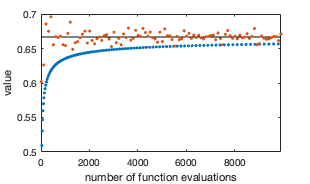
\includegraphics[width=0.45\textwidth]{img/C15MC.png}
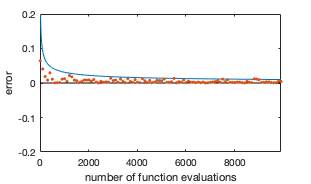
\includegraphics[width=0.45\textwidth]{img/C15MCerror.png}

\vspace{0.2cm}
\hrule
\vspace{0.2cm}

\noindent\textbf{Monte Carlo integration: other domains}
\begin{tcolorbox}
To use \textbf{Monte Carlo integration} over a region, $R$ that is not the unit box:
\begin{itemize}
\itemsep0em
    \item Create a rectangular box that encloses the region, $R$ and has area $A_{box}$. 
    \item Define the function piecewise: it will be $0$ everywhere that is outside $R$.  It will be $f(\vc{x})$ in the region $R$.
    \item To use Monte Carlo integration on the rectangular box, generate $N$ random points within the box.  Sum the function evaluated at each point and divide by $N$ to find an estimate of the average function value.  Multiply by the size of the box.

\end{itemize}

\end{tcolorbox}

% \noindent\textbf{A non-unit interval}
% \begin{enumerate}[resume=classQ]
% \item \texttt{uniform(0,5,3)} generates an array of three random numbers uniformly spaced between $0$ and $5$.  \texttt{uniform(1,5)} generates a single random number uniformly spaced between $1$ and $5$.
    
% Write Python code to generate a pair of random numbers, with one between $-1$ and $1$ and the second between $2$ and $4$.
% \vspace{1in}
% \end{enumerate}
    

\noindent\textbf{Approximating $\pi$}

Consider the following code for Monte Carlo integration.
\begin{lstlisting}   
npoints = 10**6
xyvals = uniform(0,1,[npoints,2])
indomain = (xyvals[:,0]**2+xyvals[:,1]**2)<1
integral = 4*sum(indomain)/npoints
\end{lstlisting}
\begin{enumerate}[resume=classQ]
\item Answer the following questions about the code above.
\begin{parts}
\item What is the range of $x$ being used?  What about $y$?
\vspace{1cm}

\item What is the set of $(x,y)$ for which the function will be nonzero (so $x$ and $y$ are \texttt{indomain})
\vspace{1cm}
\item Identify the region of integration.
\vspace{1cm}
\item Given the final value is \texttt{4*sum(indomain)/npoints}, what is the function of integration?
\end{parts}
\end{enumerate}

%Let $f(x,y) = 4$.  Let $R$ be the region in the first quadrant where $x^2+y^2\leq 1$.  $\displaystyle\int_R f(x,y) dA = \int_0^{\pi/2}\int_0^1 4r\ dr\ d\theta = \pi$.



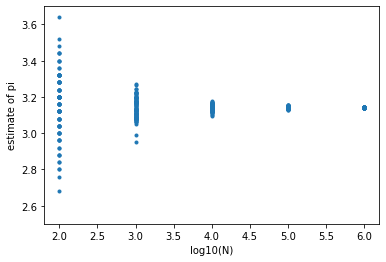
\includegraphics[width=0.5\linewidth]{img/C17piest.png}
%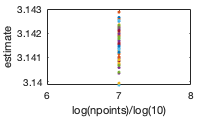
\includegraphics{img/C15MCpi7.png}
\vspace{0.1cm}

\noindent\textbf{Circular region with non-uniform function}
\begin{enumerate}[resume=classQ]
    \item Approximate the integral of a function that is not uniform: let $f(x,y) = xy$.
    
    \texttt{def fc(x,y): return x*y}
    
    Let $R$ again be the region in the first quadrant where $x^2+y^2\leq 1$.
    

    
    How would you modify the code at the top of the page to incorporate this nonuniform function?
\end{enumerate}

% \vspace{1in}

% \noindent\textbf{Example}

% %\begin{tabular}{p{12cm} c }
% Provide pseudocode for using Monte-Carlo integration to approximate the area, $\int_R dA$, where $R$ is the crescent shape shown. %&

% 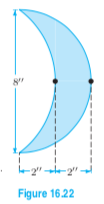
\includegraphics[scale=0.65]{img/C16crescent.png}
% %\end{tabular}



\end{document}